\documentclass[10pt]{mypackage}

% sans serif font:
%\usepackage{cmbright}
%\usepackage{sfmath}
%\usepackage{bbold} %better blackboard bold

%serif font + different blackboard bold for serif font
\usepackage{newpxtext,eulerpx}
\renewcommand*{\mathbb}[1]{\varmathbb{#1}}
\renewcommand*{\hbar}{\hslash}

\pagestyle{fancy} %better headers
\fancyhf{}
\rhead{Avinash Iyer}
\lhead{Ordinary Differential Equations: Homework 3}

\setcounter{secnumdepth}{0}

\begin{document}
\RaggedRight
\section{Part 1}%
\subsection{1.6, Problem 2}%
\begin{align*}
  \frac{dy}{dt} &= y^2 - 4y - 12\\
                &= \left(y-6\right)\left(y+2\right).
\end{align*}
We can see that $\frac{dy}{dt} = 0$ at $y=6$ and $y=-2$. Additionally, for $y > 6$, $\frac{dy}{dt} > 0$, for $y < -2$, $\frac{dy}{dt} > 0$, and for $y\in (6,2)$, $\frac{dy}{dt} < 0$. Thus, we get the following phase line.
\begin{center}
  \begin{tikzpicture}[scale=0.5]
    \draw[thick] (0,-3) -- (0,7);
    \filldraw (0,6) circle (2pt);
    \filldraw (0,-2) circle (2pt);
    \node[anchor = west] at (0,6) {$y=6$};
    \node[anchor = west] at (0,-2) {$y=-2$};
    \draw[->] (0,6) -- (0,6.5);
    \draw[->] (0,2) -- (0,1.5);
    \draw[->] (0,-3) -- (0,-2.5);
  \end{tikzpicture}
\end{center}
The equilibrium point at $y=-2$ is a sink, while the equilibrium point at $y=6$ is a source.
\subsection{1.6, Problem 7}%
\begin{align*}
  \frac{dv}{dt} &= -v^2 - 2v - 2\\
                &= -\left(v^2 + 2v + 2\right)\\
                &= -\left(\left(v+1\right)^2 + 1\right).
\end{align*}
Thus, we can see that it is never the case that $v = 0$, and that $\frac{dv}{dt} < 0$ for all $v$. The analytical solution is as follows:
\begin{align*}
  \frac{dv}{dt} &-= -\left(\left(v+1\right)^2 + 1\right)\\
  \int \frac{dv}{\left(v+1\right)^2 + 1} &= -\int dt\\
  \arctan\left(v+1\right) &= -t + C\\
  v+1 &= \tan\left(-t + C\right)\\
  v &= \tan\left(-t + C\right) - 1.
\end{align*}
\subsection{1.6, Problem 8}%
\begin{align*}
  \frac{dw}{dt} &= 3w^3 - 12w^2\\
                &= 3w^2 \left(w-2\right)\left(w+2\right).
\end{align*}
We can see that $\frac{dw}{dt} = 0$ at $w = 0$, $w = 2$, and $w = -2$. Additionally, we can see that $\frac{dw}{dt} > 0$ for $w > 2$ and $w < -2$, and $\frac{dw}{dt} < 0$ for $w\in (-2,2)$. Thus, the phase line is as follows.
\begin{center}
  \begin{tikzpicture}
    \draw[thick] (0,-4) -- (0,4);
    \filldraw (0,2) circle (2pt);
    \filldraw (0,-2) circle (2pt);
    \filldraw (0,0) circle (2pt);
    \node[anchor = west] at (0,2) {$y=2$};
    \node[anchor = west] at (0,-2) {$y=-2$};
    \node[anchor = west] at (0,0) {$y=0$};
    \draw[->] (0,2) -- (0,2.5);
    \draw[->] (0,-3) -- (0,-2.5);
    \draw[->] (0,1) -- (0,0.5);
    \draw[->] (0,-0.5) -- (0,-1);
  \end{tikzpicture}
\end{center}
The equilibrium point at $y=-2$ is a sink, the equilibrium point at $y=2$ is a source, and the equilibrium point at $y=0$ is a node.
\subsection{1.6, Problem 19}%
\begin{center}
  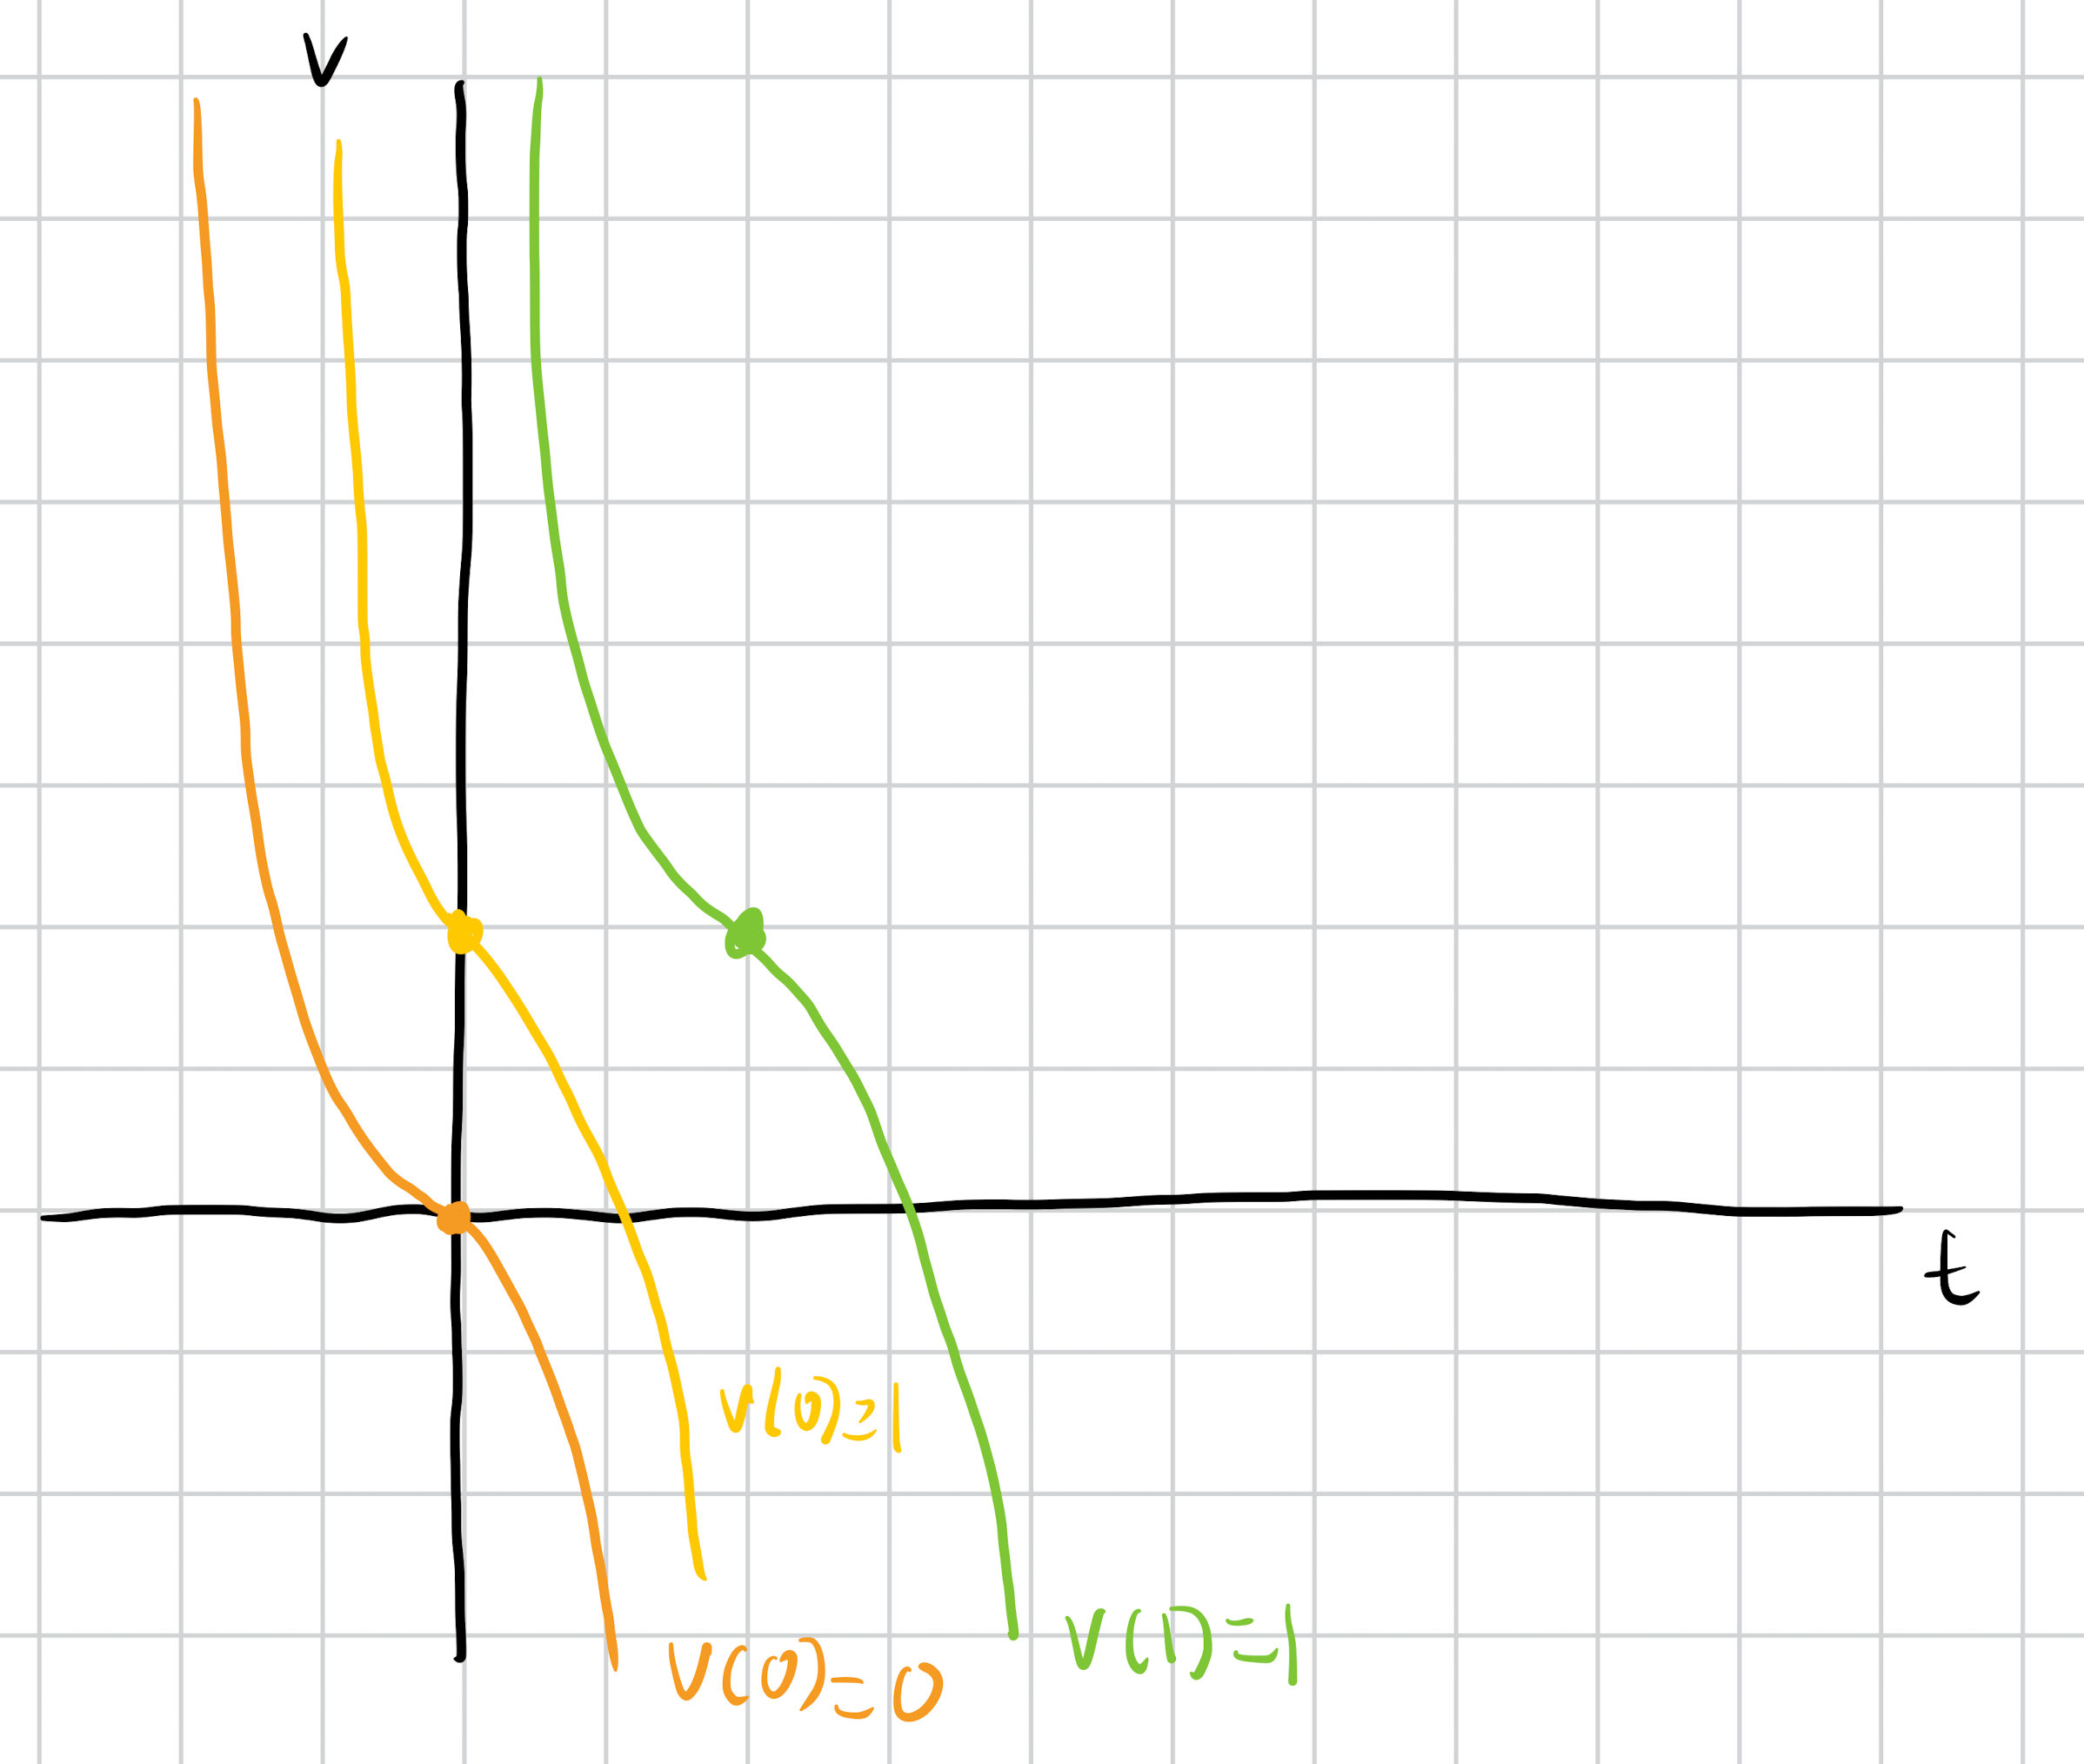
\includegraphics[width=10cm]{images/1_6_19.png}
\end{center}
\subsection{1.6, Problem 20}%
\begin{center}
  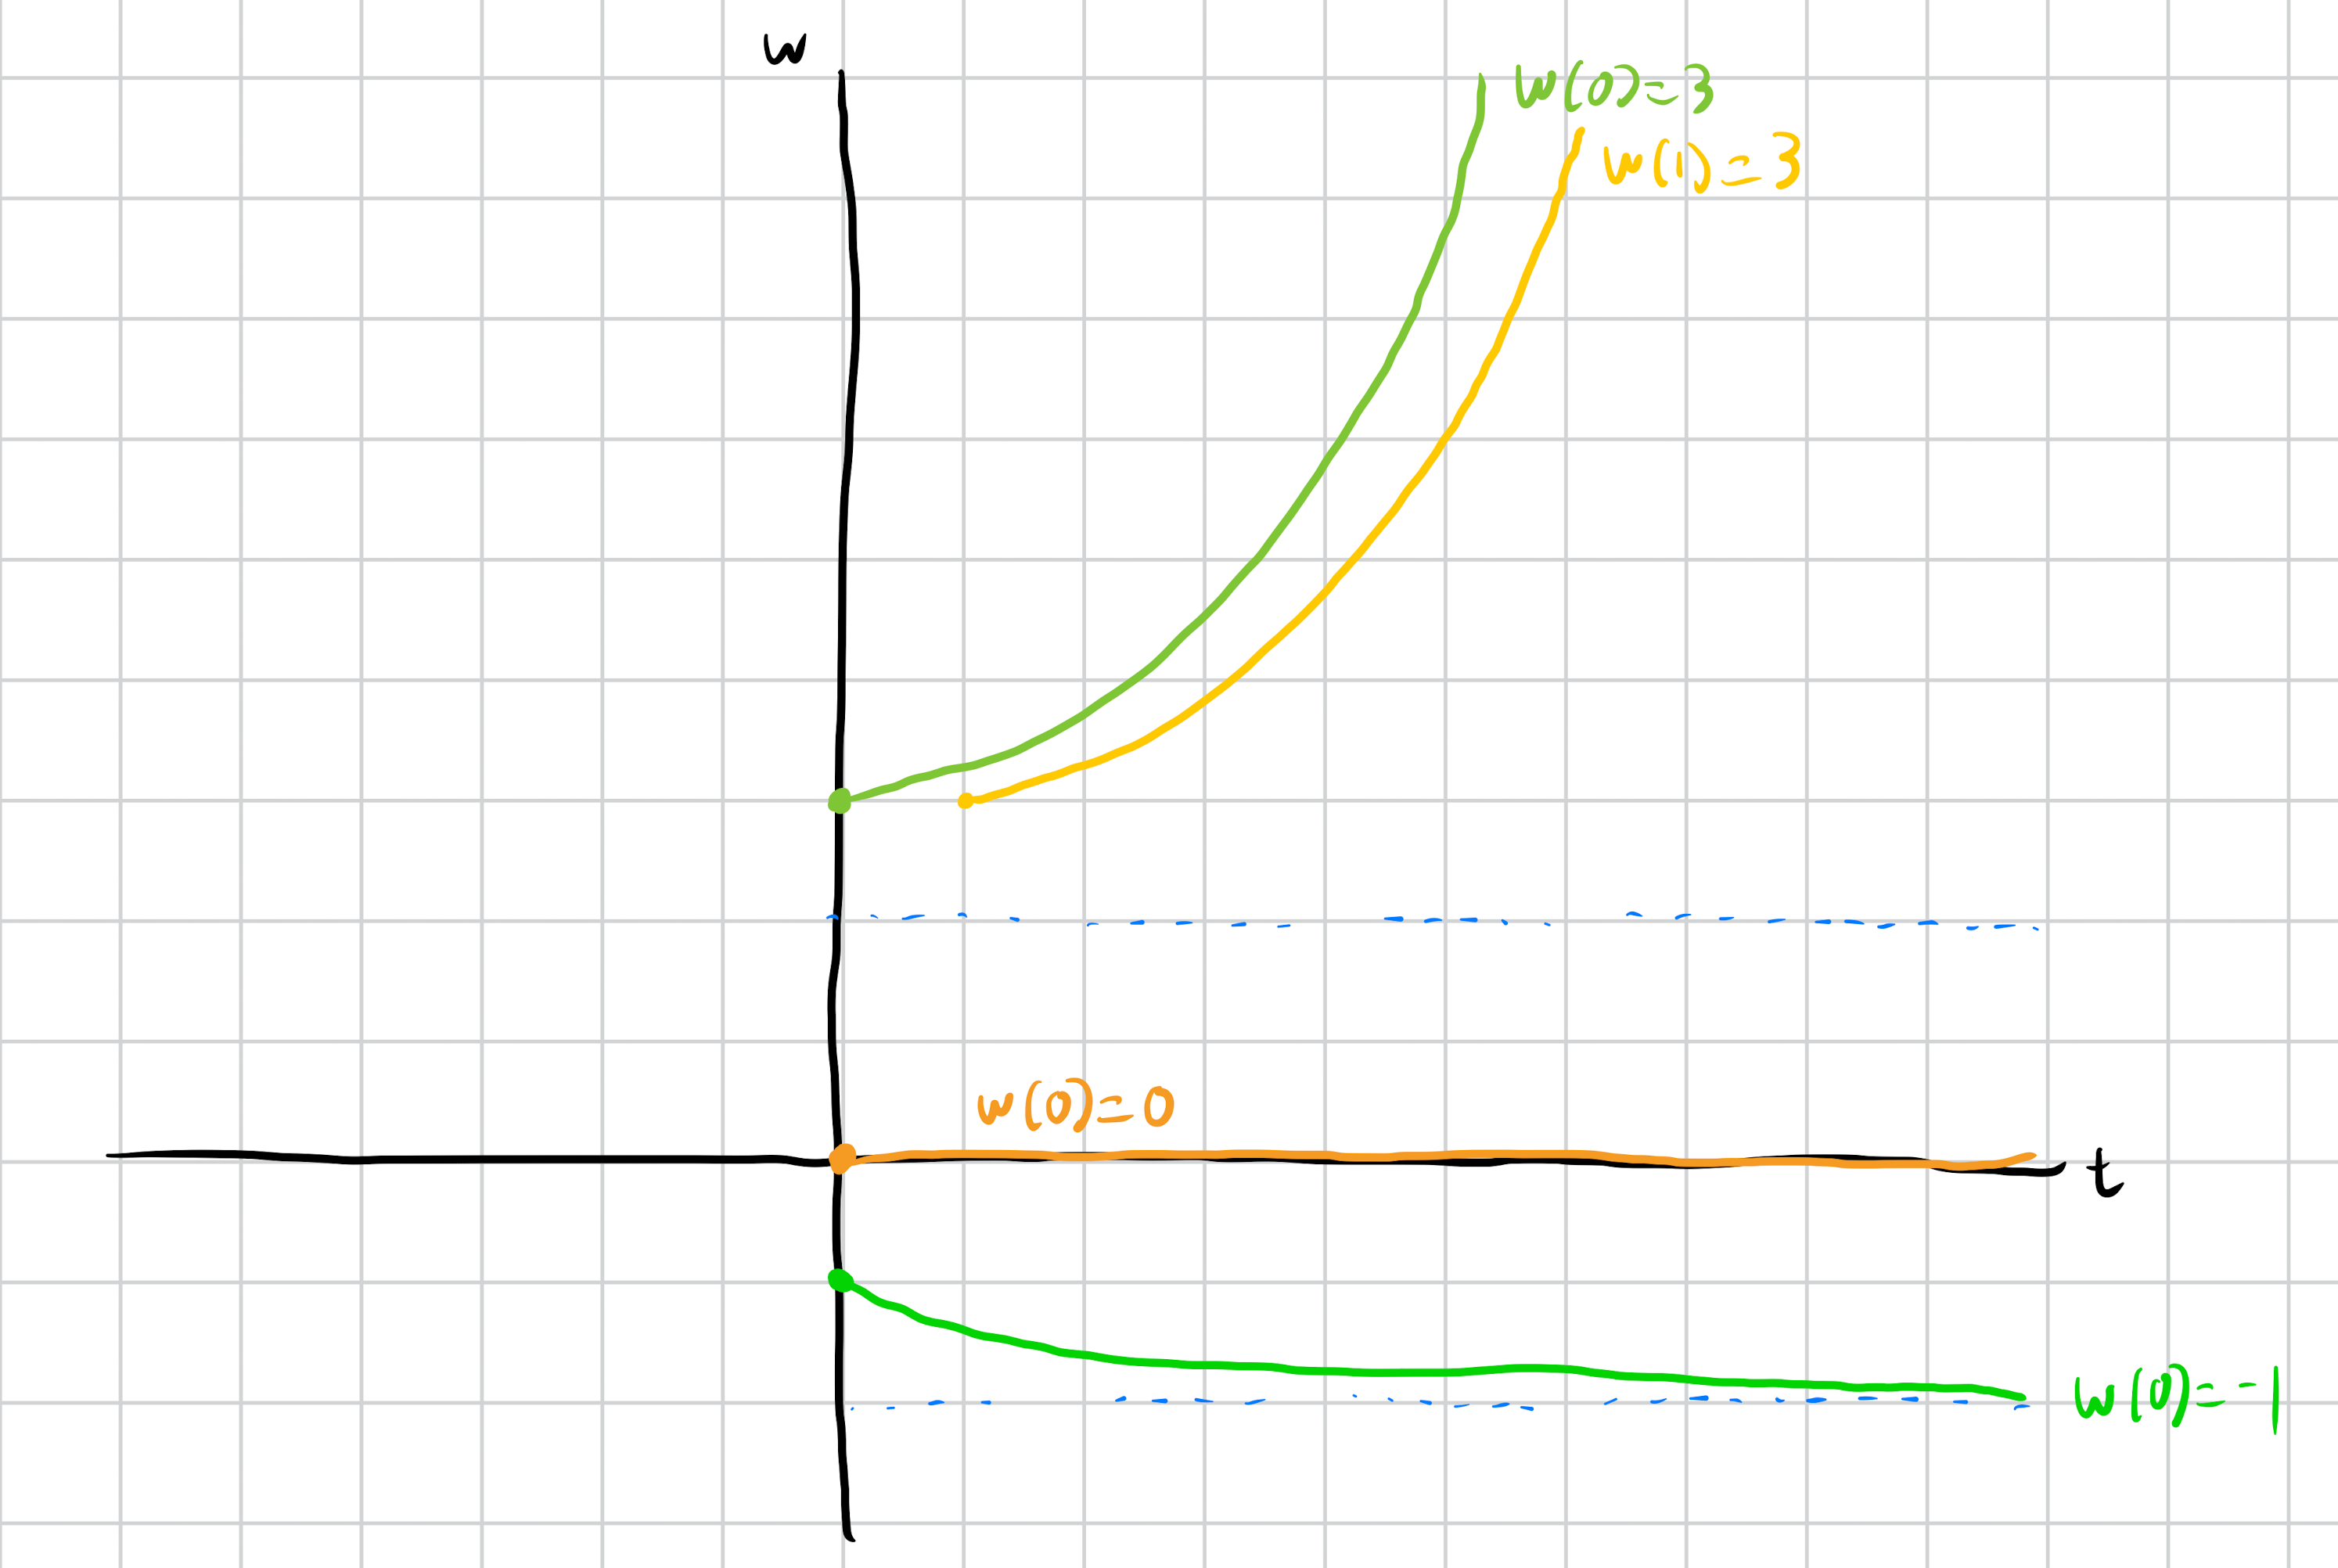
\includegraphics[width=10cm]{images/1_6_20.png}
\end{center}
\subsection{1.6, Problem 30}%
\begin{center}
  \begin{tikzpicture}
    \draw[thick] (0,0) -- (0,4);
    \filldraw (0,1) circle (2pt);
    \filldraw (0,3) circle (2pt);
    \node[anchor = west] at (0,1) {$y_1$};
    \node[anchor = west] at (0,3) {$y_2$};
    \draw[->] (0,4) -- (0,3.5);
    \draw[->] (0,1) -- (0,0.5);
    \draw[->] (0,1.5) -- (0,2);
  \end{tikzpicture}
\end{center}
\subsection{1.6, Problem 31}%
\begin{center}
  \begin{tikzpicture}
    \draw[thick] (0,0) -- (0,7);
    \filldraw (0,1) circle (2pt);
    \filldraw (0,3) circle (2pt);
    \filldraw (0,5) circle (2pt);
    \node[anchor = west] at (0,1) {$y_1$};
    \node[anchor = west] at (0,3) {$y_2$};
    \node[anchor = west] at (0,5) {$y_3$};
    \draw[->] (0,5) -- (0,5.5);
    \draw[->] (0,3.5) -- (0,4);
    \draw[->] (0,2.5) -- (0,2);
    \draw[->] (0,0) -- (0,0.5);
  \end{tikzpicture}
\end{center}
\subsection{1.6, Problem 41}%
\begin{enumerate}[(a)]
  \item The phase line is is qualitatively similar for $a > 0$ and $a < 0$; in the former case the phase line has zero equilibrium solutions, while in the latter case, the phase line has two equilibrium solutions.
  \item The phase line shifts when $a = 0$, as it has only one equilibrium solution for $a = 0$.
\end{enumerate}
\section{Part 2}%
\subsection{1.7, Problem 3}%
\subsection{1.7, Problem 6}%
\subsection{1.7, Problem 18}%

\end{document}
